\documentclass{article}
\usepackage{hyperref}
\usepackage{tabularx}
\usepackage{graphicx}
\usepackage{enumerate}
\usepackage{listings}
\usepackage{float}

\begin{document}

\title{11-792 Project Report}

\author{Nicholas Gekakis, Boyue Li}

\maketitle

\section{Overview}

In this project, we are building a distributed question answering pipeline framework,
which allows users to easily configure multiple modules,
create complex pipelines and tune parameters automatically.

\section{Requirements}

    \subsection{Easy to configure and deploy}
    The framework should be easy to configure and deploy.

    \subsection{Save and resume}
    The framework should be save intermediate results so that it can be interrupted resume running at a later time.

    \subsection{Automatical parameter tuning}
    The framework should be able to automatically tune some parameters that have been exposed to the system by the pipeline developers.
    \subsection{Load balancing}
    The framework should be able to handle load balancing since different modules require different excution time.

    \subsection{Easy to develop users' modules}
    The framwork should support a easy way for users to develop their own modules.

\section{Design}

    \subsection{Overview}

    As shown in Fig. \ref{fig:control_flow},
    a pipeline is constructed from several independent modules.
    A module reads data from data server,
    processes data according to all possible parameters,
    then save results for each configuration to the data server.

    The number of instances of each module is managed by the load balancing server.

    \begin{figure}[h]
        \begin{center}
            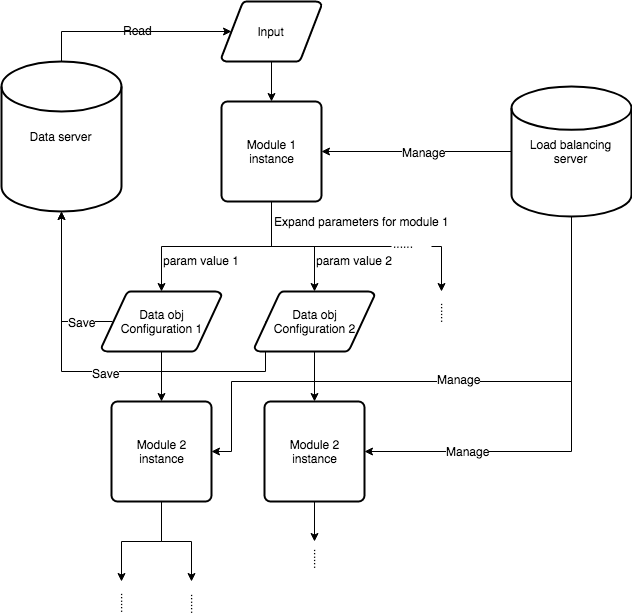
\includegraphics[width=\textwidth]{fig/control_flow.png}
        \end{center}
        \label{fig:control_flow}
        \caption{Control flowchart.}
    \end{figure}

    \begin{figure}[h]
        \begin{center}
            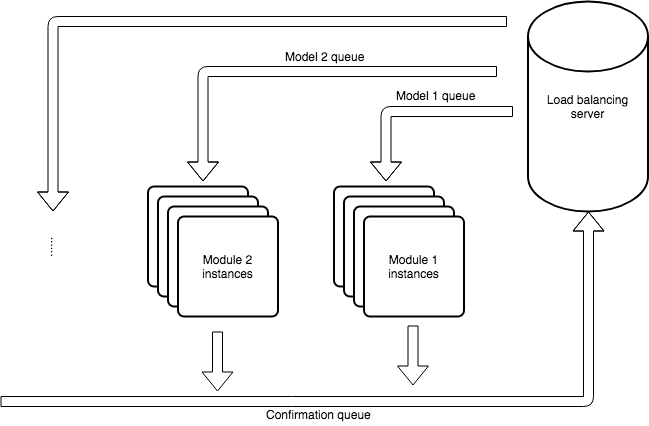
\includegraphics[width=\textwidth]{fig/information_flow.png}
        \end{center}
        \label{fig:information_flow}
        \caption{Information flowchart.}
    \end{figure}


    Every module runs on an independent process,
    and communicates through RabbitMQ using data objects which contains parameters, current excuetion status and the path to input file.
    Fig. \ref{fig:information_flow} describes the information flow.
    Load balancing server distributes jobs to different modules' instances.
    Once the job is finished, the instance send a confirmation to the load balancing server.


    Users only need to specify
    \begin{enumerate}
        \item The connections between modules
        \item The parameters every module needs
    \end{enumerate}
    The framework will automatically handle execution, load balancing and parameter tuning.

    \begin{figure}[H]
        \begin{center}
            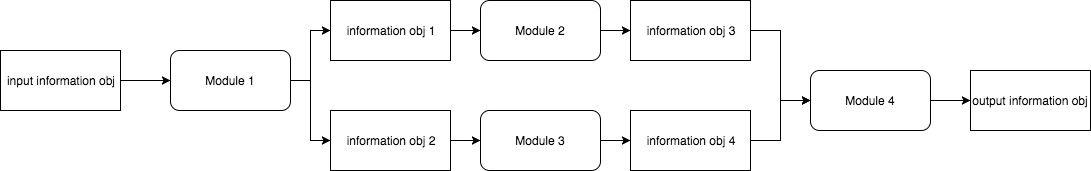
\includegraphics[width=1.2\textwidth]{fig/sample_pipeline.png}
        \end{center}
        \label{fig:sample_pipeline}
        \caption{A sample pipeline}
    \end{figure}
    Figure \ref{fig:sample_pipeline} shows a sample pipeline which passes the input information object
    through some modules and produces the output information object.

    We also provide an command line executable, to ease users' pain of coding.


    \subsection{Pipeline}
    The pipeline class manages modules and parameters.
    It reads configuration file, creates the pipeline and controls load balancing when running.

    \begin{figure}[h]
        \begin{center}
            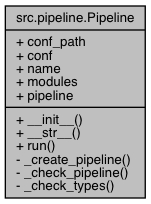
\includegraphics[width=0.3\textwidth]{fig/pipeline_uml.png}
        \end{center}
        \label{fig:pipeline_uml}
        \caption{UML diagram for the pipeline class.}
    \end{figure}

    \subsection{Module}
    A module is the basic computation unit which takes an input and produces an output.
    Every input and output is an information object defined in sec. \ref{sec:infomation_object}.

    A module needs to maintain the following fileds:
    \begin{itemize}
        \item Name of the module.
        \item Input module.
        \item Output module.
        \item Parameters.
        \item Number of instances.
        \item Configuration of the pipeline.
    \end{itemize}

    \begin{figure}[H]
        \begin{center}
            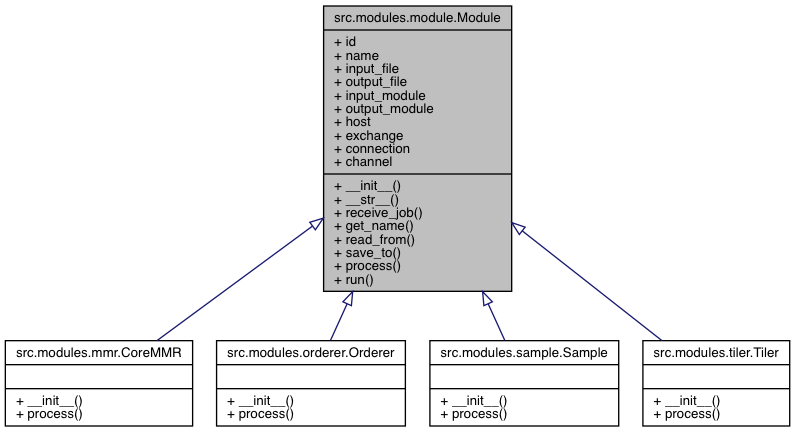
\includegraphics[width=\textwidth]{fig/module_uml.png}
        \end{center}
        \label{fig:module_uml}
        \caption{UML diagrams for the abstract module class and derived classes.}
    \end{figure}

    \subsection{Parameter}
    \label{sec:parameter}
    The parameter class manages one parameter.
    It should handle all operations related the parameter,
    including updating the parameter value according to its step size,
    set and reset the value.

    It also needs to save maintain the following fileds:
    \begin{itemize}
        \item Name of the parameter.
        \item Default values of the parameter.
        \item Tuning interval of the parameter.
        \item Step size of the parameter.
    \end{itemize}

    \begin{figure}[H]
        \begin{center}
            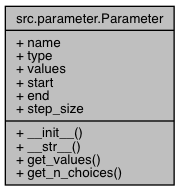
\includegraphics[width=0.3\textwidth]{fig/param_uml.png}
        \end{center}
        \label{fig:param_uml}
        \caption{UML diagram for parameter class.}
    \end{figure}

    \subsection{Job}
    \label{sec:infomation_object}
    The job class is the information object used to pass jobs between modules.
    It maintains the following fileds:
    \begin{itemize}
        \item Producing module: the module that produced this information object.
        \item Consuming module: the module that this information object to be passed to.
        \item Data path: the path to actual data file.
        \item Configuration: the configuration that produced the data object.
    \end{itemize}


    \begin{figure}[H]
        \begin{center}
            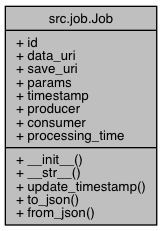
\includegraphics[width=0.3\textwidth]{fig/job_uml.png}
        \end{center}
        \label{fig:job_uml}
        \caption{UML diagram for job class.}
    \end{figure}


    \subsection{File format}
    A data file has a description contains the following fileds:
    \begin{itemize}
        \item Data: the actual data.
        \item Configuration: the configuration produced the file it.
        \item Timestamp: the timestamp when it is created.
        \item Producing module: the module that produced this file.
    \end{itemize}


    \subsection{Configuration file}
    We use YAML files to configure the framework.

    \subsection{Executable}
    We provide an executable that reads in the configuration file, and runs all possible configurations.

\section{Implemented Modules}

    Table \ref{tbl:modules} listed all modules and their parameters we implemented.

    \begin{table}[h]
        \centering
        \begin{tabular}{|l|l|}
            \hline
            Module  & Parameters \\ \hline
            CoreMMR &            \\ \hline
            Orderer &            \\ \hline
            Tiler   &            \\ \hline
            Rouge   &            \\ \hline
        \end{tabular}
        \caption{Table of implemented modules.}
        \label{tbl:modules}
    \end{table}

\section{Example pipeline}
    \subsection{Toy example}
    This pipeline consists of three sample modules,
    which do nothing but add it own configuration and parameters to the data to show this pipeline is working.

    \begin{figure}[H]
        \begin{center}
            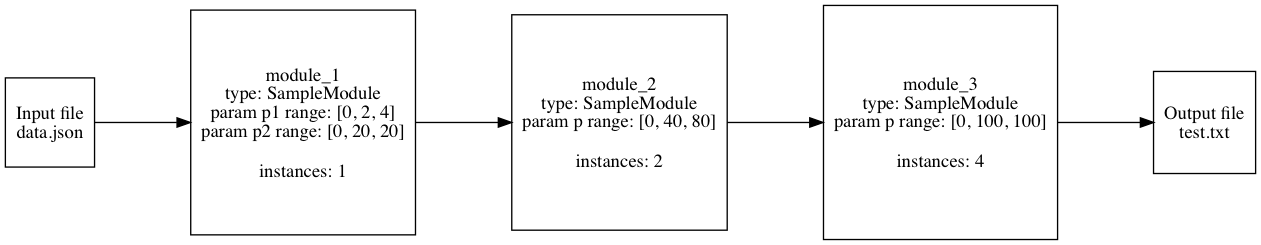
\includegraphics[width=\textwidth]{fig/toy_pipeline.png}
        \end{center}
        \label{fig:toy_pipeline}
        \caption{The structure for toy pipeline}
    \end{figure}


    \subsection{BioAsq example}
    This pipeline is a fully operational BioAsq pipeline.

    \begin{figure}[H]
        \begin{center}
            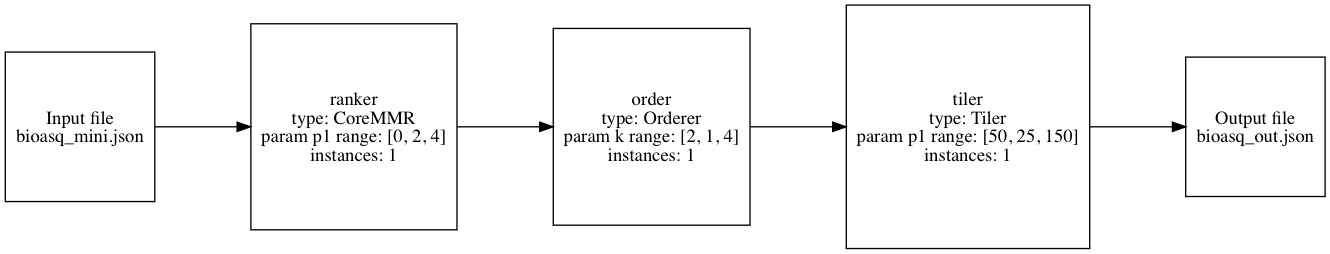
\includegraphics[width=\textwidth]{fig/bioasq_pipeline.png}
        \end{center}
        \label{fig:bioasq_pipeline}
        \caption{The structure for BioAsq pipeline}
    \end{figure}


\section{Experiments}
    \subsection{Dataset}
    The results were run on a subset (100 total questions) of the bioasq_train_formatted.json dataset.
    \subsection{Results}
    Our experimental results show that the best configuration uses the following parameters: alpha=0.65, k=2, word_limit=100.

\section{Conclusion}

\section*{Acknowledgements}

\end{document}
